\documentclass[9pt,aspectratio=1610]{beamer}
\usepackage{booktabs}% better quality tables, https://ctan.org/pkg/booktabs
\usepackage{multirow}
\usepackage{array}%    additional options for table columns, https://ctan.org/pkg/array
\usepackage{tikz}
\usepackage{tikz-3dplot}
\tikzset{>=latex} % for LaTeX arrow head
\usetikzlibrary{decorations.pathmorphing} % for snake
\usetikzlibrary{matrix}
\usepackage{amsmath}
\usepackage[table]{xcolor}
\usepackage{arydshln}
\usepackage{caption}
\usepackage{subcaption}
\usepackage{hyperref}
\usepackage{cite}
%\usepackage[style=ieee,maxbibnames=10,sorting=none,backend=biber]{biblatex}
%\addbibresource{./refs.bib}

\captionsetup{labelformat=simple}
\hypersetup{
	colorlinks=true,
	linkcolor=blue,
	citecolor=blue,
	urlcolor=blue
}

\newcommand{\hl}[1]{\textbf{\color{structure}#1}}

%%%
\usetheme{CambridgeUS}
\usecolortheme{dolphin}
\usefonttheme{professionalfonts}
\usefonttheme[onlymath]{serif}
\setbeamerfont{title}{series=\bfseries}
%\setbeamercolor{title}{fg=white,bg=darkred}
\setbeamercolor{frametitle}{fg=black}
\setbeamerfont{caption}{size=\tiny}
\setbeamertemplate{enumerate items}[default]
\setbeamertemplate{bibliography item}{\insertbiblabel}
\AtBeginSection[]{
	\begin{frame}
		\vfill
		\centering
		\begin{beamercolorbox}[sep=8pt,center,shadow=true,rounded=true]{title}
			\usebeamerfont{title}\thesection.  \insertsectionhead\par%
		\end{beamercolorbox}
		\vfill
	\end{frame}
}
%%%

%%% booktabs
\renewcommand{\arraystretch}{1.5}
%%%

\title{Approval Talk [HIG-23-005]\\``Search for rare decays of the Higgs boson into a photon and a \(\rho^0\), \(\phi\) or \(K^{*0}\) meson"}
\author[K. Yoon]{R. Covarelli\textsuperscript{1} \and M. Pelliccioni\inst{1} \and G. Umoret\inst{1}\\
	\and M. D'Alfonso\inst{2} \and G. Gomez Ceballos\inst{2} \and C. Paus\inst{2} \and \underline{K. Yoon}\inst{2}}
\institute[MIT]{\textsuperscript{1}Politecnico di Torino, Turin, Italy \and \inst{2} Massachusetts Institute of Technology, Cambridge, U.S.}
\date{March ??, 2024}
\begin{document}

% Title
\begin{frame}[plain]
    \maketitle
\end{frame}

% Intro
\begin{frame}{Documentation}
	\begin{itemize}
		\item Collaboration of \textbf{MIT} and \textbf{Torino} groups, targeting different categories.
		\item CADI \href{https://cms.cern.ch/iCMS/analysisadmin/cadilines?id=2681&ancode=HIG-23-005&tp=an&line=HIG-23-005}{HIG-23-005}
		\item Three analysis notes (two separate + one combined):\\
		\textbf{AN-22-004} (MIT, v9), \textbf{AN-22-067} (Torino, v10), and \textbf{AN-23-004} (combined, v7)
		\item Q\&A with ARC, L3, and L2 conveners: \href{https://twiki.cern.ch/twiki/bin/viewauth/CMS/HMesonGamma_QA}{Twiki Q\&A}
	\end{itemize}
\end{frame}

% Motivations (table)
\begin{frame}{Motivations}
	\begin{itemize}
		\item SM prediction of branching ratios of \(H\rightarrow \phi\gamma\) or \(\rho\gamma\) within reasonable reach (??)
		\item ATLAS upper limit at \(95\)\% CL is \(\mathcal{O}(10^{-4})\) to \(\mathcal{O}(10^{-3})\).
		\item \(K^*_0\) channel added as an extension of ditrack + gamma final state analyses.
	\end{itemize}
	\footnotesize
	\begin{table}[!ht]
		\centering
		\begin{tabular}[t]{|l|c|c|l|l|}
			\hline
			\multicolumn{1}{|c|}{\cellcolor{lightgray}\small Channel} & \cellcolor{lightgray}\small Coupling & \cellcolor{lightgray}\small SM \(\mathcal{BR}(H\rightarrow M\gamma)\) & \multicolumn{1}{c|}{\cellcolor{lightgray}\small Limits on \(\mathcal{BR}\)} & \multicolumn{1}{c|}{\cellcolor{lightgray}\small Notes} \\
			\hline
			
			% phi
			\multirow{2}{*}{\(H\rightarrow \phi\gamma\)} & \multirow{2}{*}{\(s\)} & \multirow{2}{*}{\((1.68\pm0.8) \times 10^{-5}\)\cite{K_nig_2015}} & Exp. \(4.2^{+1.8}_{-1.2}\times10^{-4}\) & ATLAS Run 2, \(35.6\;\textrm{fb}^{-1}\) \\ & & & Obs. \(5.0\times10^{-4}\) \cite{ATLAS_rhophigamma2023} & \(\phi\gamma\rightarrow K^+K^-\gamma\)\\
			\hline
			
			% rho
			\multirow{2}{*}{\(H\rightarrow \rho\gamma\)} & \multirow{2}{*}{\(u, d\)} & \multirow{2}{*}{\((2.31\pm0.11) \times 10^{-6}\)\cite{K_nig_2015}} & Exp. \(10.0^{+4.9}_{-2.8}\times10^{-4}\) & ATLAS Run 2, \(35.6\;\textrm{fb}^{-1}\) \\ & & & Obs. \(10.4\times10^{-4}\) \cite{ATLAS_rhophigamma2023} & \(\rho\gamma\rightarrow \pi^+\pi^-\gamma\) \\
			\hline
			
			% K0star
			\multirow{2}{*}{\(H\rightarrow K^*_0\gamma\)} & & \tiny (Only available for \(H\rightarrow d\bar{s} + \bar{d}s\)) & Exp. \(3.7^{+1.5}_{-1.0}\times10^{-4}\) & ATLAS Run 2, \(134\;\textrm{fb}^{-1}\) \\ & \multirow{-2}{*}{\(d\&s\) (flavor-changing)} & \(1.19\times10^{-11}\) \cite{Aranda_2020} & Obs. \(2.2\times10^{-4}\) \cite{ATLAS_omegaK0stargamma} & \(K^*_0\gamma\rightarrow K^\pm\pi^\mp\gamma\) \\
			\hline
		\end{tabular}
		\label{tab:Higgs_rare_decays}
	\end{table}
\end{frame}

% Motivations (direct, indirect)
\begin{frame}{Motivations}
	
	\(H \rightarrow M \gamma \) \cite{K_nig_2015}
	\begin{itemize}
		\item \textbf{Direct contribution}. The Higgs couples via Yukawa coupling to the quarks, one of which radiates a photon.
		\item \textbf{Indirect contribution}. The off-shell \(\gamma^*\) or \(Z^*\) produced in \(H\rightarrow \gamma\gamma^*, \gamma Z^*\) \textit{fragments} into a meson.
	\end{itemize}
	Direct and indirect contributions interfere destructively. Due to light quark masses, direct contribution is smaller than indirect. Direct contribution is sensitive to deviation from SM Higgs couplings. Branching ratios are \(\mathcal{O}(10^{-5}\textup{--}10^{-6})\).
	\begin{figure}[t!]
		\centering
		\begin{subfigure}[t]{0.48\linewidth}
			\centering
			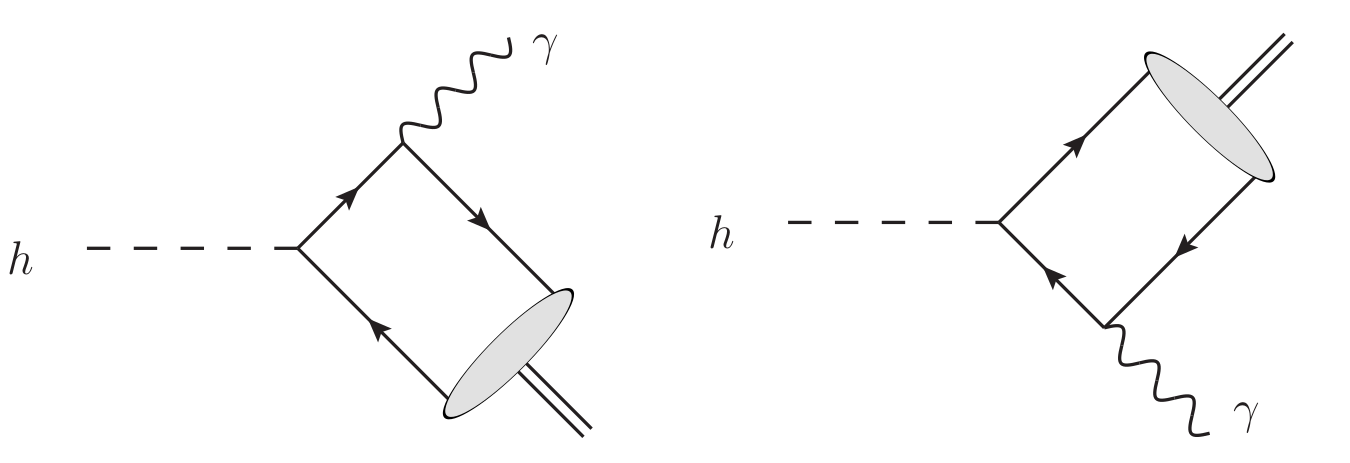
\includegraphics[height=1.2in]{figures/Higgs_phirhoomega_direct.png}
			\caption{Direct contributions via Yukawa coupling to the light quarks.}
		\end{subfigure}
		\hfill
		\begin{subfigure}[t]{0.48\linewidth}
			\centering
			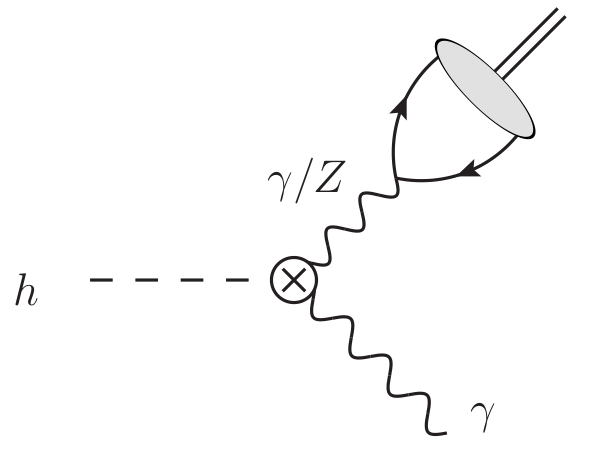
\includegraphics[height=1.2in]{figures/Higgs_phirhoomega_indirect.png}
			\caption{Indirect contribution via a virtual photon or \(Z\) boson.}
		\end{subfigure}
		\caption{Leading order Feynman diagrams to the \(H\rightarrow M\gamma\) processes. Image taken from Fig. 2 of \cite{K_nig_2015}.}
	\end{figure}
\end{frame}

% Strategy 
\begin{frame}{Strategy}
	\begin{itemize}
		\item \hl{Final states}
		\begin{enumerate}
			\item High energy \textbf{photon}
			\item High energy \textbf{ditrack} from meson
			\begin{align*}
				\phi(1020)&\rightarrow K^+K^-\;\;(\mathrm{BR} \sim 49\%)\\
				\rho(770)&\rightarrow \pi^+\pi^-\;\;(\mathrm{BR} \sim 100\%)\\
				K^*_0(700)&\rightarrow K^\pm\pi^\mp\;\;(\mathrm{BR} \sim 100\%)
			\end{align*}
		\end{enumerate}
	\end{itemize}
\end{frame}

\begin{frame}{Strategy}
	\begin{itemize}
		\item \hl{Production}
		\vspace{1em}
		\begin{columns}
			\centering
			\begin{column}{0.31\textwidth}
				\centering
				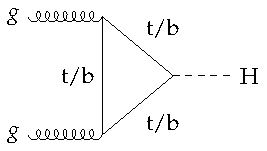
\includegraphics[height=0.25\textheight]{feynman-diagrams/ggH.pdf}\\
				\textbf{ggH}
			\end{column}
			\begin{column}{0.31\textwidth}
				\centering
				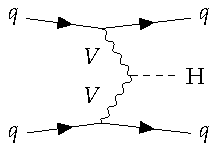
\includegraphics[height=0.25\textheight]{feynman-diagrams/VBF.pdf}\\
				\textbf{VBF}
			\end{column}
			\begin{column}{0.31\textwidth}
				\centering
				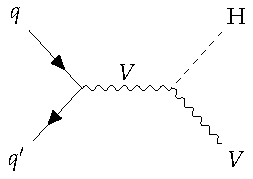
\includegraphics[height=0.25\textheight]{feynman-diagrams/VH.pdf}\\
				\textbf{VH}
			\end{column}
		\end{columns}
	\end{itemize}
\end{frame}

\begin{frame}{Bibliography}
	\scriptsize
	\bibliographystyle{JHEP}
	\bibliography{refs.bib}
\end{frame}
\end{document}
